\documentclass[aspectratio=169,11pt]{beamer}

% ================================================================
% "TABIIY TILNI QAYTA ISHLASH" KURSI
% MA'RUZA 3 --- Vektor fazo modellari, semantik munosabatlar va
%               ularni vizualizatsiya qilish
%              (d03_vektor_embedding.tex)
% Arxetiplar: [A][B][C][D][E] + 4 bo'lim [F][G][H][I][J][K][L] +
%             [M][N][O][P][Q][R] + ilova [S]
% Rendered slayd soni: ~40 (4 kichik mavzuli rasmiy ma'ruza --- L1/L2 istisno precedentiga mos)
% Qulflangan [I2]: cos(a,b)=2/3~0.667 --- P3 (4-kun) birinchi assert manbayi.
%   Korpus: course_map.yaml hand_example verbatim:
%     a=(1,1,1,0) "nlp juda qiziq", b=(1,1,0,1) "nlp juda foydali",
%     V=(nlp, juda, qiziq, foydali)
% ================================================================

% ================================================================
% RANGLAR  (asl fayldan o'zgarishsiz)
% ================================================================
\definecolor{cnublue}{rgb}{0.07,0.14,0.62}
\definecolor{cnubluelight}{rgb}{0.18,0.30,0.72}
\definecolor{cnubluebg}{rgb}{0.90,0.92,0.97}
\definecolor{deepblue}{rgb}{0.07,0.14,0.62}
\definecolor{deepred}{rgb}{0.60,0.00,0.00}
\definecolor{deepgreen}{rgb}{0.00,0.45,0.00}
\definecolor{halfgray}{gray}{0.55}

% ================================================================
% BEAMER MAVZU --- Boadilla + maxsus footer  (asl fayldan o'zgarishsiz)
% ================================================================
\usetheme{Boadilla}
\newcommand{\ctx}[2]{%
  \fcolorbox{#1!60!black}{#1!12}{\scriptsize\strut #2}%
}
\providecommand{\uzq}{\textquotesingle{}}
\setbeamercolor{structure}{fg=cnublue}
\setbeamercolor{frametitle}{bg=cnublue,fg=white}
\setbeamercolor{title}{bg=cnublue,fg=white}
\setbeamercolor{block title}{bg=cnublue,fg=white}
\setbeamercolor{block body}{bg=cnubluebg,fg=black}
\setbeamercolor{alerted text}{fg=deepred}
\setbeamercolor{author in head/foot}{bg=cnubluelight,fg=white}
\setbeamercolor{section in head/foot}{bg=cnublue,fg=white}
\setbeamercolor{page number in head/foot}{bg=cnubluelight,fg=white}

\setbeamertemplate{mini frame}{}
\setbeamertemplate{mini frame in current section}{}
\setbeamertemplate{mini frame in current subsection}{}
\setbeamertemplate{headline}{}
\setbeamertemplate{navigation symbols}{}

\setbeamertemplate{footline}{%
  \leavevmode%
  \hbox{%
    \begin{beamercolorbox}[wd=0.17\paperwidth,ht=2.5ex,dp=1.25ex,leftskip=0.5em]{author in head/foot}%
      \usebeamerfont{author in head/foot}\scriptsize\insertshortauthor%
    \end{beamercolorbox}%
    \begin{beamercolorbox}[wd=0.69\paperwidth,ht=2.5ex,dp=1.25ex,center]{section in head/foot}%
      \usebeamerfont{section in head/foot}%
      \scriptsize\insertsectionnavigationhorizontal{0.69\paperwidth}{}{}%
    \end{beamercolorbox}%
    \begin{beamercolorbox}[wd=0.14\paperwidth,ht=2.5ex,dp=1.25ex,rightskip=0.5em]{page number in head/foot}%
      \hfill\scriptsize\color{white}%
      \insertframenumber{}/\inserttotalframenumber%
    \end{beamercolorbox}%
  }%
  \vskip0pt%
}

% ================================================================
% PAKETLAR  (asl fayldan o'zgarishsiz)
% ================================================================
\usepackage[utf8]{inputenc}
\usepackage[T1]{fontenc}
\usepackage{lmodern}
\usepackage{amsmath,amssymb}
\usepackage{booktabs}
\usepackage{array}
\usepackage{xcolor}
\usepackage{listings}
\lstset{
    language=Python,
    basicstyle=\ttfamily\scriptsize,
    keywordstyle=\bfseries\color{deepblue},
    emphstyle=\ttfamily\color{deepred},
    stringstyle=\color{deepgreen},
    commentstyle=\itshape\color{halfgray},
    numbers=none,
    numberstyle=\scriptsize\color{halfgray},
    rulesepcolor=\color{cnublue!30},
    frame=shadowbox,
    breaklines=true,
    showstringspaces=false,
    columns=fullflexible,
    keepspaces=true,
    tabsize=2
}
\usepackage{tcolorbox}
\tcbuselibrary{skins}
\tcbset{
  defbox/.style={colback=cnubluebg,colframe=cnublue,
                 fonttitle=\small\bfseries\color{white},
                 attach boxed title to top left={yshift=-2mm,xshift=4mm},
                 boxed title style={colback=cnublue,colframe=cnublue}},
  warnbox/.style={colback=orange!8,colframe=orange!70!black,
                  fonttitle=\small\bfseries},
  okbox/.style={colback=green!7,colframe=green!55!black,
                fonttitle=\small\bfseries}
}
\usepackage{tikz}
\usetikzlibrary{arrows.meta,positioning,calc,angles,quotes,backgrounds,%
                decorations.pathreplacing,intersections}
\usepackage{pgfplots}
\pgfplotsset{compat=1.18}

% ----------------------------------------------------------------
% INTUITSIYA GRAFIKLARI UCHUN QAYTA ISHLATILADIGAN USLUBLAR
% (ilmiy rahbar tavsiyasi: har bir formula yonida intuitiv grafik)
% ----------------------------------------------------------------
\tikzset{
  axisline/.style={->,thick,draw=halfgray},
  vecA/.style={->,very thick,draw=cnublue,>=Stealth},
  vecB/.style={->,very thick,draw=deepred,>=Stealth},
  vecRel/.style={->,very thick,draw=deepgreen,>=Stealth},
  vecGhost/.style={->,very thick,draw=deepgreen!55,
                   dash pattern=on 3pt off 2pt,>=Stealth},
  ghostline/.style={draw=halfgray,dash pattern=on 2pt off 2pt},
  dotpt/.style={circle,inner sep=1.6pt},
}
% kichik izoh sarlavhasi (grafik tagidagi bir qatorlik intuitsiya)
\newcommand{\gcap}[1]{{\scriptsize\color{halfgray}#1}}

% ================================================================
% QO'SHIMCHALAR  (asl fayldan o'zgarishsiz)
% ================================================================
\AtBeginSection[]{%
  \begin{frame}{Prezentatsiya rejasi}
    \tableofcontents[currentsection]
  \end{frame}}

\newcommand{\bunda}[1]{{\small\textbf{bunda:}\; #1}}
\newcommand{\bajarildi}{{\color{deepgreen}\large$\checkmark$}\;}

% ================================================================
% METAMA'LUMOT
% ================================================================
\title[Vektor fazo va embeddinglar]{Vektor fazo modellari, embeddinglar va semantik munosabatlar}
\subtitle{Tabiiy tilni qayta ishlash --- 3-ma'ruza}
\author[A.A.\,Abdulali]{A.A.\,Abdulali}
\date{18-iyun 2026}
\institute{11:00--12:20 \quad$\cdot$\quad mavzu \textnumero{}3}

% ================================================================
\begin{document}
% ================================================================

% ----------------------------------------------------------------
% [A] TITUL
% ----------------------------------------------------------------
\maketitle

% ================================================================
\section[Kirish]{Kirish: TF-IDF (Term Frequency--Inverse Document Frequency) dan embeddinggacha}
% ================================================================

% ----------------------------------------------------------------
% [B] TAKRORLASH: L2 va bugungi P2 dan ikki savol
% ----------------------------------------------------------------
\begin{frame}{Takrorlash: oldingi amaliyotda nima qurdik?}
  \begin{columns}[T]
    \begin{column}{0.49\textwidth}
      \begin{tcolorbox}[warnbox,title=1-savol]
        \small
        2-amaliyotda sentiment klassifikatori \textbf{nima} ustida ishladi ---
        xom matn ustidami yoki vektor ustida?\\[3pt]
        \footnotesize Vektorni qaysi usul yaratdi?
      \end{tcolorbox}
    \end{column}
    \begin{column}{0.49\textwidth}
      \begin{tcolorbox}[warnbox,title=2-savol]
        \small
        TF-IDF fazosida \texttt{"qiziq"} va \texttt{"qiziqarli"}
        so'zlari bir-biriga \textbf{qanchalik yaqin}?
      \end{tcolorbox}
    \end{column}
  \end{columns}
  \pause
  \vspace{4pt}
  \begin{columns}[T]
    \begin{column}{0.49\textwidth}
      \begin{tcolorbox}[okbox,title=1-javob]
        \small
        Vektor ustida --- \textbf{TF-IDF / BoW} matritsasi.
        Model xom matnni emas, sonli vektorni ko'radi.
      \end{tcolorbox}
    \end{column}
    \begin{column}{0.49\textwidth}
      \begin{tcolorbox}[okbox,title=2-javob]
        \small
        \textbf{Umuman yaqin emas!} Ular ikki \textbf{alohida ustun} ---
        o'xshashligi $0$.\\
        \footnotesize\textcolor{halfgray}{TF-IDF so'z ma'nosini bilmaydi. Bugun shuni hal qilamiz.}
      \end{tcolorbox}
    \end{column}
  \end{columns}
\end{frame}

% ----------------------------------------------------------------
% [C] BUGUNGI MAQSADLAR
% ----------------------------------------------------------------
% ----------------------------------------------------------------
% [C] BUGUNGI MAQSADLAR
% ----------------------------------------------------------------
\begin{frame}{Bugungi dars maqsadlari}
\small
\begin{enumerate}\setlength\itemsep{6pt}
    \item Distributiv gipoteza asosida so\textquotesingle{}z embeddingi nima uchun
          kerakligini tushuntirasiz.

    \item TF-IDF vektorlarining semantik cheklovini
          \textit{qiziq}--\textit{qiziqarli} misolida izohlaysiz.

    \item Ikki vektor orasidagi kosinus o\textquotesingle{}xshashligini
          qo\textquotesingle{}lda hisoblab,
          $\cos(a,b)=\frac{2}{3}$ natijasini talqin qilasiz.

    \item Vektor arifmetikasidan foydalanib so\textquotesingle{}z analogiyasi uchun
          $t=\mathbf{b}-\mathbf{a}+\mathbf{c}$ maqsad vektorini tuzasiz.

    \item \texttt{cosine\_similarity}, \texttt{most\_similar}
          funksiyalari va PCA natijasini matematik jihatdan izohlaysiz.
\end{enumerate}

\vfill

\begin{tcolorbox}[defbox]
\footnotesize
Minimum talablar: 1-ma\textquotesingle{}ruzadagi BoW va TF-IDF vektorlari;
vektor, skalyar ko\textquotesingle{}paytma va Evklid normasi.
\end{tcolorbox}
\end{frame}

% ----------------------------------------------------------------
% [D] REJA VA VAQT BYUDJETI
% ------------------------------------------------

% ----------------------------------------------------------------
% [E] MUAMMO BIRINCHI: TF-IDF MA'NONI USHLAMAYDI
% ----------------------------------------------------------------
% ----------------------------------------------------------------
% BUGUNGI MUAMMO
% ----------------------------------------------------------------
\begin{frame}{Bugungi darsda yechiladigan muammo}
\small

\begin{columns}[T,totalwidth=\textwidth]
  \begin{column}{0.52\textwidth}
    \textbf{1-ma\textquotesingle{}ruzadan qolgan savol:}

    \vspace{3pt}
    TF-IDF stemming yoki lemmatizatsiyasiz
    \textit{qiziq} va \textit{qiziqarli} so\textquotesingle{}zlarini
    ma\textquotesingle{}nan yaqin deb ko\textquotesingle{}ra oladimi?

    \vspace{6pt}

    \begin{tcolorbox}[alertbox,title=Javob: yo\textquotesingle{}q]
      \footnotesize
      Lug\textquotesingle{}atda ular ikki alohida o\textquotesingle{}lcham sifatida turadi:
      \[
        \textit{qiziq}\rightarrow(1,0), \qquad
        \textit{qiziqarli}\rightarrow(0,1)
      \]
      Kosinus o\textquotesingle{}xshashligi: $\cos=0$.
    \end{tcolorbox}
  \end{column}

  \begin{column}{0.44\textwidth}
    \textbf{Muammoning mohiyati:}

    \vspace{3pt}
    \begin{itemize}\setlength\itemsep{5pt}
      \item TF-IDF so\textquotesingle{}z shakllarini alohida belgi sifatida ko\textquotesingle{}radi.
      \item Semantik bog\textquotesingle{}liqlik bevosita kodlanmaydi.
      \item Sinonimlar ajralib qoladi:
            \textit{avtomobil} $\ne$ \textit{mashina}.
    \end{itemize}

    \vspace{5pt}

    \begin{tcolorbox}[defbox,title=Yechim]
      \footnotesize
      Zich vektor — \textit{embedding}: so\textquotesingle{}zni kichik
      o\textquotesingle{}lchamli vektor bilan ifodalaydi. Ma\textquotesingle{}nosi
      yaqin so\textquotesingle{}zlar fazoda yaqin joylashadi.
    \end{tcolorbox}
  \end{column}
\end{columns}

\end{frame}

% ================================================================
\section[Embeddinglar]{Zich vektorlar: so'z embeddinglari}
% ================================================================

% ----------------------------------------------------------------
% [F1] INTUITSIYA: SIYRAK VS ZICH
% ----------------------------------------------------------------
\begin{frame}{So\textquotesingle{}zni raqamli vektorga qanday aylantiramiz?}
\footnotesize

\begin{columns}[T,totalwidth=\textwidth]
%------------------------------------------------
\begin{column}{0.50\textwidth}

\textbf{Siyrak ifoda: one-hot / TF-IDF}

\vspace{2pt}
\[
\textit{nlp}\rightarrow (0,\ldots,1,\ldots,0)
\]

\begin{itemize}\setlength\itemsep{3pt}
    \item Vektor uzunligi lug\textquotesingle{}at hajmiga teng: $|V|$.
    \item Ko\textquotesingle{}p komponentalari nol bo\textquotesingle{}ladi.
    \item Semantik yaqinlik bevosita ifodalanmaydi.
\end{itemize}

\vspace{4pt}

\textbf{Zich ifoda: embedding}

\vspace{2pt}
\[
\textit{nlp}\rightarrow (0.21,-0.08,0.66,\ldots)
\]

\begin{itemize}\setlength\itemsep{3pt}
    \item Odatda kichik o\textquotesingle{}lchamli: $d \ll |V|$.
    \item Qiymatlar matndan o\textquotesingle{}rganiladi.
    \item Ma\textquotesingle{}nosi yaqin so\textquotesingle{}zlar fazoda yaqinlashadi.
\end{itemize}

\end{column}
%------------------------------------------------
\begin{column}{0.46\textwidth}

\begin{tcolorbox}[defbox,title=Distributiv gipoteza]
\footnotesize
So\textquotesingle{}zning ma\textquotesingle{}nosi uning qanday
kontekstlarda uchrashi orqali shakllanadi.
\end{tcolorbox}

\vspace{3pt}

\textbf{Misol:} \textit{choy} va \textit{kofe} ko\textquotesingle{}pincha
o\textquotesingle{}xshash kontekstlarda keladi.

\vspace{5pt}

\begin{tabular}{@{}l l@{}}
\textit{choy} & \ctx{blue}{issiq}\ \ctx{green!60!black}{ichdim}\ \ctx{orange}{finjon} \\
[5pt]
\textit{kofe} & \ctx{blue}{issiq}\ \ctx{green!60!black}{ichdim}\ \ctx{orange}{finjon}
\end{tabular}

\vspace{7pt}

\begin{tcolorbox}[alertbox,title=Xulosa]
\footnotesize
TF-IDF so\textquotesingle{}zning uchrashiga tayanadi, embedding esa
uning kontekstini ham hisobga oladi.
\end{tcolorbox}

\end{column}
%------------------------------------------------
\end{columns}

\end{frame}

% ----------------------------------------------------------------
% [G1] RASMIY TA'RIF: EMBEDDING
% ----------------------------------------------------------------
\begin{frame}{So\textquotesingle{}z embeddingi: rasmiy ta\textquotesingle{}rif}
\footnotesize

\begin{tcolorbox}[defbox]
\textbf{Embedding} — lug\textquotesingle{}atdagi har bir so\textquotesingle{}zni
kichik o\textquotesingle{}lchamli zich vektorga akslantiruvchi
o\textquotesingle{}rganilgan funksiya:
\[
    E: V \rightarrow \mathbb{R}^{d}, \qquad d \ll |V|.
\]
\end{tcolorbox}

\vspace{2pt}

\begin{columns}[T,totalwidth=\textwidth]
\begin{column}{0.46\textwidth}
\textbf{Belgilashlar}
\begin{itemize}\setlength\itemsep{3pt}
    \item $V$ — lug\textquotesingle{}at;
    \item $|V|$ — lug\textquotesingle{}at hajmi;
    \item $d$ — embedding o\textquotesingle{}lchami;
    \item $E(w)=\mathbf{e}_w$ — $w$ so\textquotesingle{}zining vektori.
\end{itemize}

\vspace{3pt}

\textbf{Taqqoslash}
\[
\text{one-hot: } d=|V|,\qquad
\text{embedding: } d\ll |V|.
\]
\end{column}

\begin{column}{0.50\textwidth}
\centering
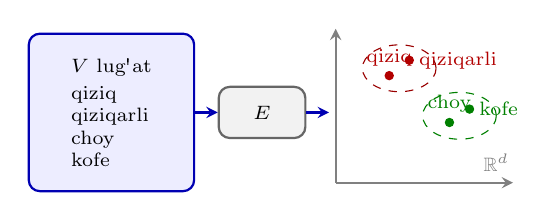
\begin{tikzpicture}[>=stealth,scale=0.85, every node/.style={font=\scriptsize}]
  % Vocabulary box
  \node[draw=blue!70!black, thick, rounded corners,
        fill=blue!7, minimum width=2.1cm, minimum height=2.0cm,
        align=left] (vocab) at (0,0)
  {$V$ lug\textquotesingle{}at\\[2pt]
   qiziq\\
   qiziqarli\\
   choy\\
   kofe};

  % Embedding function
  \node[draw=black!60, thick, rounded corners,
        fill=gray!10, minimum width=1.1cm, minimum height=0.65cm] (E) at (2.25,0)
  {$E$};

  % Semantic space
  \draw[->, thick, gray] (3.35,-1.05) -- (6.0,-1.05);
  \draw[->, thick, gray] (3.35,-1.05) -- (3.35,1.25);
  \node[gray] at (5.75,-0.75) {$\mathbb{R}^{d}$};

  % Points
  \fill[red!70!black] (4.15,0.55) circle (2pt);
  \node[red!70!black, above] at (4.15,0.55) {qiziq};

  \fill[red!70!black] (4.45,0.78) circle (2pt);
  \node[red!70!black, right] at (4.45,0.78) {qiziqarli};

  \fill[green!50!black] (5.05,-0.15) circle (2pt);
  \node[green!50!black, above] at (5.05,-0.15) {choy};

  \fill[green!50!black] (5.35,0.05) circle (2pt);
  \node[green!50!black, right] at (5.35,0.05) {kofe};

  % Arrows
  \draw[->, thick, blue!70!black] (vocab.east) -- (E.west);
  \draw[->, thick, blue!70!black] (E.east) -- (3.25,0);

  % clusters
  \draw[dashed, red!60!black] (4.30,0.66) ellipse (0.55 and 0.35);
  \draw[dashed, green!50!black] (5.20,-0.05) ellipse (0.55 and 0.35);
\end{tikzpicture}

\vspace{3pt}

\begin{tcolorbox}[alertbox,title=Asosiy g\textquotesingle{}oya]
\footnotesize
So\textquotesingle{}zlar alohida ustunlar emas, balki
umumiy semantik fazodagi yaqin yoki uzoq nuqtalar sifatida qaraladi.
\end{tcolorbox}
\end{column}
\end{columns}

\end{frame}


% ----------------------------------------------------------------
% [G2] QANDAY O'RGANILADI: WORD2VEC, GLOVE, FASTTEXT
% ----------------------------------------------------------------
\begin{frame}{Embeddinglar qanday o\textquotesingle{}rganiladi? Uch asosiy yondashuv}
\footnotesize

\begin{center}
\begin{tabular}{p{0.20\textwidth} p{0.42\textwidth} p{0.28\textwidth}}
\toprule
\textbf{Yondashuv} & \textbf{Asosiy g\textquotesingle{}oya} & \textbf{O\textquotesingle{}zbek tili uchun izoh} \\
\midrule
\textbf{Word2Vec} &
So\textquotesingle{}z va uning atrofidagi kontekst orasidagi bog\textquotesingle{}liqlikni o\textquotesingle{}rganadi. CBOW va Skip-gram usullari ishlatiladi. &
Korpus yetarli bo\textquotesingle{}lsa, tez va amaliy. \\[3pt]

\textbf{GloVe} &
So\textquotesingle{}zlarning butun korpus bo\textquotesingle{}yicha birga uchrashish statistikasidan foydalanadi. &
Katta va toza korpus talab qiladi. \\[3pt]

\textbf{FastText} &
So\textquotesingle{}zni belgilar n-gramlari yig\textquotesingle{}indisi sifatida ifodalaydi. &
Agglutinativ tillar va yangi so\textquotesingle{}zlar uchun foydali. \\
\bottomrule
\end{tabular}
\end{center}

\vspace{5pt}

\begin{tcolorbox}[defbox]
\footnotesize
\textbf{Bu ma\textquotesingle{}ruzada e\textquotesingle{}tibor nimaga qaratiladi?}

\vspace{2pt}
Embeddinglarni o\textquotesingle{}qitish tafsilotlariga hozircha chuqur kirmaymiz.
Asosiy maqsad — tayyor vektorlar orqali o\textquotesingle{}xshashlikni hisoblash,
so\textquotesingle{}z analogiyalarini tushuntirish va PCA yordamida ularni vizual
ko\textquotesingle{}rsatish.
\end{tcolorbox}

\end{frame}

% ----------------------------------------------------------------
\begin{frame}{Nega one-hot vektorlar ma\textquotesingle{}noni to\textquotesingle{}liq ifodalay olmaydi?}
\small

\textbf{1-qadam.} Ikki har xil so\textquotesingle{}zning one-hot vektorlari:

\[
\textit{qiziq}\rightarrow \mathbf{u}=(1,0,0,\ldots),
\qquad
\textit{qiziqarli}\rightarrow \mathbf{v}=(0,1,0,\ldots)
\]

\vspace{4pt}

\textbf{2-qadam.} Skalyar ko\textquotesingle{}paytmani hisoblaymiz:

\[
\mathbf{u}\cdot \mathbf{v}
=1\cdot0+0\cdot1+\cdots=0.
\]

\vspace{4pt}

\textbf{3-qadam.} Demak, one-hot fazosida ikki har xil so\textquotesingle{}zning
o\textquotesingle{}xshashligi odatda $0$ chiqadi — ma\textquotesingle{}nosi yaqin
bo\textquotesingle{}lsa ham.

\vspace{6pt}

\begin{tcolorbox}[defbox]
\footnotesize
\textbf{Xulosa:} one-hot ifoda so\textquotesingle{}zlarni alohida ustunlar sifatida
ko\textquotesingle{}radi. Shu sababli semantik yaqinlik bevosita ifodalanmaydi.
Embedding esa ma\textquotesingle{}nosi yaqin so\textquotesingle{}zlarni fazoda
bir-biriga yaqinlashtirishga xizmat qiladi.
\end{tcolorbox}

\end{frame}

\begin{frame}{Qo\textquotesingle{}lda misol: bir xil so\textquotesingle{}zlar, ikki xil ifoda}
\footnotesize

\begin{columns}[T,totalwidth=\textwidth]
%================================================
\begin{column}{0.48\textwidth}
\centering
\textbf{One-hot: siyrak ifoda}

\vspace{3pt}
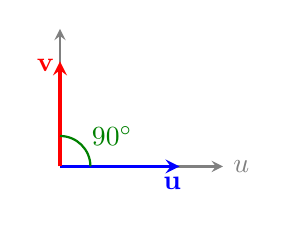
\begin{tikzpicture}[scale=0.92,>=stealth]
  \draw[->,thick,gray] (0,0) -- (2.25,0) node[right] {$u$};
  \draw[->,thick,gray] (0,0) -- (0,1.9);
  \draw[->,very thick,blue] (0,0) -- (1.65,0);
  \draw[->,very thick,red]  (0,0) -- (0,1.45);
  \draw[green!50!black,thick] (0.42,0) arc (0:90:0.42);
  \node[green!50!black] at (0.72,0.42) {$90^\circ$};
  \node[blue] at (1.55,-0.23) {$\mathbf{u}$};
  \node[red]  at (-0.20,1.40) {$\mathbf{v}$};
\end{tikzpicture}

\vspace{5pt}

\begin{tcolorbox}[defbox,width=\linewidth]
\[
\textit{qiziq}\rightarrow \mathbf{u}=(1,0)
\]
\[
\textit{qiziqarli}\rightarrow \mathbf{v}=(0,1)
\]
\[
\mathbf{u}\cdot\mathbf{v}=0,
\qquad
\cos(\mathbf{u},\mathbf{v})=0
\]
\end{tcolorbox}

\vspace{2pt}
\textit{Natija:} ma\textquotesingle{}nosi yaqin bo\textquotesingle{}lsa ham,
one-hot fazosida ular yaqin emas.
\end{column}

%================================================
\begin{column}{0.48\textwidth}
\centering
\textbf{Embedding: zich ifoda}

\vspace{3pt}
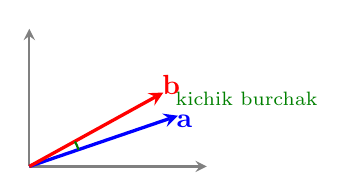
\begin{tikzpicture}[scale=0.92,>=stealth]
  \draw[->,thick,gray] (0,0) -- (2.45,0);
  \draw[->,thick,gray] (0,0) -- (0,1.9);
  \draw[->,very thick,blue] (0,0) -- (2.05,0.70);
  \draw[->,very thick,red]  (0,0) -- (1.85,1.02);
  \draw[green!50!black,thick] (0.68,0.23) arc (19:29:0.72);
  \node[green!50!black,above] at (3,0.70) {\scriptsize kichik burchak};
  \node[blue] at (2.14,0.62) {$\mathbf{a}$};
  \node[red]  at (1.96,1.13) {$\mathbf{b}$};
\end{tikzpicture}

\vspace{5pt}

\begin{tcolorbox}[defbox,width=\linewidth]
\[
\textit{qiziq}\rightarrow \mathbf{a}=(0.9,0.4)
\]
\[
\textit{qiziqarli}\rightarrow \mathbf{b}=(0.8,0.5)
\]
\[
\mathbf{a}\cdot\mathbf{b}
=0.9\cdot0.8+0.4\cdot0.5=0.92
\]
\end{tcolorbox}

\vspace{2pt}
\textit{Natija:} sifatli embeddingda ma\textquotesingle{}nosi yaqin
so\textquotesingle{}zlar fazoda ham yaqin joylashadi.
\end{column}
%================================================
\end{columns}

\end{frame}

\begin{frame}{Sizning vazifangiz: qaysi juft yaqinroq?}
\small

\begin{tcolorbox}[alertbox,title=Vazifa]
Distributiv gipotezaga ko\textquotesingle{}ra, yaxshi o\textquotesingle{}qitilgan
embedding fazosida qaysi juft so\textquotesingle{}z bir-biriga yaqinroq
bo\textquotesingle{}lishi kerak?

\vspace{3pt}
\[
\text{(a) }(\textit{avtomobil},\textit{mashina})
\qquad
\text{(b) }(\textit{avtomobil},\textit{banan})
\]
\end{tcolorbox}

\vspace{5pt}

\begin{columns}[T,totalwidth=\textwidth]
\begin{column}{0.46\textwidth}
\textbf{To\textquotesingle{}g\textquotesingle{}ri javob:}

\vspace{3pt}
\[
(\textit{avtomobil},\textit{mashina})
\]

\footnotesize
Chunki bu ikki so\textquotesingle{}z ko\textquotesingle{}pincha o\textquotesingle{}xshash
kontekstlarda uchraydi: \textit{haydadi}, \textit{sotib oldi},
\textit{ta\textquotesingle{}mirladi}.
\end{column}

\begin{column}{0.50\textwidth}
\textbf{Kontekstlar orqali asoslash:}

\vspace{3pt}
\footnotesize
\begin{tabular}{@{}l l@{}}
\textit{avtomobil} & haydadi, sotib oldi, ta\textquotesingle{}mirladi \\
\textit{mashina}   & haydadi, sotib oldi, ta\textquotesingle{}mirladi \\
\textit{banan}     & yedi, meva, sariq \\
\end{tabular}

\vspace{7pt}

\begin{tcolorbox}[defbox]
\footnotesize
\textbf{Xulosa:} kontekstlari o\textquotesingle{}xshash so\textquotesingle{}zlarning
embedding vektorlari odatda yaqin joylashadi.
\end{tcolorbox}
\end{column}
\end{columns}

\end{frame}

\section[Kosinus]{Kosinus o'xshashligi(cosine similarity)}
% ================================================================

% ----------------------------------------------------------------
% [F2] INTUITSIYA: BURCHAK
% ----------------------------------------------------------------
\begin{frame}{Intuitsiya: o\textquotesingle{}xshashlik — vektorlar orasidagi burchak}
\small

\begin{columns}[T,totalwidth=\textwidth]
%------------------------------------------------
\begin{column}{0.46\textwidth}
\centering
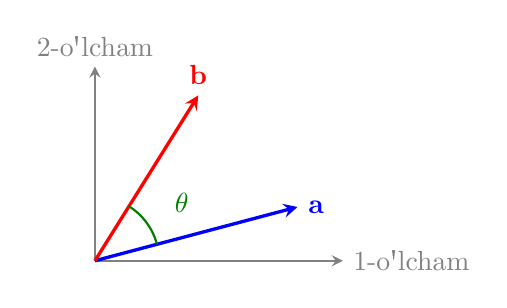
\begin{tikzpicture}[scale=1.05,>=stealth]
  \draw[->,thick,gray] (0,0) -- (3.0,0) node[right] {1-o\textquotesingle{}lcham};
  \draw[->,thick,gray] (0,0) -- (0,2.35) node[above] {2-o\textquotesingle{}lcham};

  \draw[->,very thick,blue] (0,0) -- (2.45,0.65) node[right] {$\mathbf{a}$};
  \draw[->,very thick,red]  (0,0) -- (1.25,2.0) node[above] {$\mathbf{b}$};

  \draw[green!50!black,thick] (0.75,0.20) arc (15:58:0.78);
  \node[green!50!black] at (1.05,0.70) {$\theta$};
\end{tikzpicture}

\vspace{6pt}

\begin{tcolorbox}[defbox,width=0.95\linewidth]
\footnotesize
Kosinus o\textquotesingle{}xshashligi vektorlarning uzunligini emas,
ular orasidagi \textbf{yo\textquotesingle{}nalish yaqinligini} baholaydi.
\end{tcolorbox}
\end{column}

%------------------------------------------------
\begin{column}{0.50\textwidth}
\textbf{Asosiy g\textquotesingle{}oya}

\vspace{4pt}
\begin{itemize}\setlength\itemsep{5pt}
  \item Har bir so\textquotesingle{}z yoki hujjat fazodagi vektor sifatida qaraladi.
  \item Burchak kichik bo\textquotesingle{}lsa, vektorlar o\textquotesingle{}xshash yo\textquotesingle{}nalishda.
  \item Burchak $90^\circ$ ga yaqin bo\textquotesingle{}lsa, bog\textquotesingle{}liqlik kuchsiz.
\end{itemize}

\vspace{6pt}

\footnotesize
\textbf{Nega uzunlik emas?}\\
Bir mavzudagi qisqa va uzun matnlarning vektor uzunligi farq qilishi mumkin.
Kosinus esa ularning yo\textquotesingle{}nalishini solishtiradi.
\end{column}
\end{columns}

\end{frame}

% ----------------------------------------------------------------
% [G2] RASMIY TA'RIF: KOSINUS + BUNDA
% ----------------------------------------------------------------
\begin{frame}{Kosinus o\textquotesingle{}xshashligi: rasmiy ta\textquotesingle{}rif}
\small

\begin{tcolorbox}[defbox]
\[
\cos(\mathbf{a},\mathbf{b})
=
\frac{\mathbf{a}\cdot\mathbf{b}}
{\|\mathbf{a}\|\,\|\mathbf{b}\|}
=
\frac{\sum_{i=1}^{n} a_i b_i}
{\sqrt{\sum_{i=1}^{n} a_i^2}\sqrt{\sum_{i=1}^{n} b_i^2}},
\qquad
\mathbf{a},\mathbf{b}\neq\mathbf{0}.
\]
\end{tcolorbox}

\vspace{2pt}

\begin{columns}[T,totalwidth=\textwidth]
\begin{column}{0.52\textwidth}
\textbf{Belgilashlar}
\begin{itemize}\setlength\itemsep{4pt}
    \item $\mathbf{a},\mathbf{b}\in\mathbb{R}^{n}$ — TF-IDF yoki embedding vektorlar;
    \item $\mathbf{a}\cdot\mathbf{b}$ — skalyar ko\textquotesingle{}paytma;
    \item $\|\mathbf{a}\|$, $\|\mathbf{b}\|$ — Evklid normalari;
    \item $n$ — vektor o\textquotesingle{}lchami.
\end{itemize}

\vspace{4pt}
\textbf{Talqin}
\begin{itemize}\setlength\itemsep{1pt}
    \item $\cos=1$ — bir xil yo\textquotesingle{}nalish;
    \item $\cos=0$ — ortogonal, umumiy yo\textquotesingle{}nalish yo\textquotesingle{}q;
    \item TF-IDF vektorlari manfiy bo\textquotesingle{}lmagani uchun qiymat odatda $[0,1]$ da bo\textquotesingle{}ladi.
\end{itemize}
\end{column}

\begin{column}{0.44\textwidth}
\centering
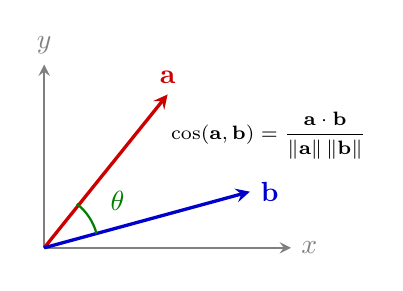
\begin{tikzpicture}[scale=0.95,>=stealth]
  \draw[->,thick,gray] (0,0) -- (3.3,0) node[right] {$x$};
  \draw[->,thick,gray] (0,0) -- (0,2.45) node[above] {$y$};

  \draw[->,very thick,red!80!black]  (0,0) -- (1.65,2.05) node[above] {$\mathbf{a}$};
  \draw[->,very thick,blue!80!black] (0,0) -- (2.75,0.75) node[right] {$\mathbf{b}$};

  \draw[green!50!black,thick] (0.70,0.19) arc (15:52:0.75);
  \node[green!50!black] at (0.98,0.63) {$\theta$};

  \node[align=center,font=\scriptsize] at (3,1.5)
  {$\displaystyle
  \cos(\mathbf{a},\mathbf{b})
  =\frac{\mathbf{a}\cdot\mathbf{b}}
  {\|\mathbf{a}\|\,\|\mathbf{b}\|}$};
\end{tikzpicture}

\vspace{5pt}

\footnotesize
Burchak kichraygan sari kosinus qiymati kattalashadi;
burchak kattalashgan sari o\textquotesingle{}xshashlik kamayadi.
\end{column}
\end{columns}

\end{frame}

\begin{frame}{Keltirib chiqarish: nega normaga bo\textquotesingle{}lamiz?}
\small

\begin{columns}[T,totalwidth=\textwidth]
%------------------------------------------------
\begin{column}{0.56\textwidth}

\textbf{1-qadam.} Skalyar ko\textquotesingle{}paytmaning geometrik ta\textquotesingle{}rifi:
\[
\mathbf{a}\cdot\mathbf{b}
=
\|\mathbf{a}\|\,\|\mathbf{b}\|\cos\theta.
\]

\vspace{4pt}

\textbf{2-qadam.} Bizga kerak bo\textquotesingle{}lgan $\cos\theta$ ni ajratamiz:
\[
\cos\theta
=
\frac{\mathbf{a}\cdot\mathbf{b}}
{\|\mathbf{a}\|\,\|\mathbf{b}\|}.
\]

\vspace{4pt}

\textbf{3-qadam.} Agar vektorni ikki marta uzaytirsak, yo\textquotesingle{}nalish o\textquotesingle{}zgarmaydi:
\[
\cos(2\mathbf{a},\mathbf{b})
=
\frac{2(\mathbf{a}\cdot\mathbf{b})}
{2\|\mathbf{a}\|\,\|\mathbf{b}\|}
=
\cos(\mathbf{a},\mathbf{b}).
\]

\end{column}

%------------------------------------------------
\begin{column}{0.40\textwidth}
\centering

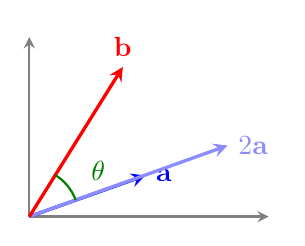
\begin{tikzpicture}[scale=0.95,>=stealth]
  \draw[->,thick,gray] (0,0) -- (3.2,0);
  \draw[->,thick,gray] (0,0) -- (0,2.4);

  \draw[->,very thick,blue] (0,0) -- (1.55,0.55) node[right] {$\mathbf{a}$};
  \draw[->,very thick,blue!45] (0,0) -- (2.65,0.95) node[right] {$2\mathbf{a}$};
  \draw[->,very thick,red]  (0,0) -- (1.25,2.0) node[above] {$\mathbf{b}$};

  \draw[green!50!black,thick] (0.62,0.22) arc (20:58:0.66);
  \node[green!50!black] at (0.92,0.61) {$\theta$};
\end{tikzpicture}

\vspace{6pt}

\begin{tcolorbox}[defbox]
\footnotesize
\textbf{Xulosa:} kosinus o\textquotesingle{}xshashligi uzunlikni emas,
vektorlarning yo\textquotesingle{}nalishini solishtiradi.
Shuning uchun u matn uzunligi turlicha bo\textquotesingle{}lganda ham qulay.
\end{tcolorbox}

\end{column}
\end{columns}

\end{frame}
% ----------------------------------------------------------------
% [I2] QO'LDA HISOB --- QULFLANGAN TRACEABILITY SLAYD
%
% P3 (kun-4) birinchi assert bilan solishtiring:
%   cos(a,b) = 2/3 ~ 0.667   [Ma'ruza L3 [I2]-slayd]
% Korpus: course_map.yaml hand_example verbatim:
%   a=(1,1,1,0) "nlp juda qiziq", b=(1,1,0,1) "nlp juda foydali"
%   V = (nlp, juda, qiziq, foydali)
% ----------------------------------------------------------------
\begin{frame}{Qo\textquotesingle{}lda hisob: ikki vektorning kosinus o\textquotesingle{}xshashligi}
\small

\begin{tcolorbox}[defbox]
\[
H_1:\ \text{``nlp juda qiziq''}\rightarrow
\mathbf{a}=(1,1,1,0),
\qquad
H_2:\ \text{``nlp juda foydali''}\rightarrow
\mathbf{b}=(1,1,0,1)
\]
\footnotesize
Lug\textquotesingle{}at tartibi:
\[
(\textit{nlp},\ \textit{juda},\ \textit{qiziq},\ \textit{foydali})
\]
\end{tcolorbox}

\vspace{3pt}

\begin{columns}[T,totalwidth=\textwidth]
\begin{column}{0.52\textwidth}
\textbf{Hisoblash}

\[
\mathbf{a}\cdot\mathbf{b}
=1\cdot1+1\cdot1+1\cdot0+0\cdot1=2
\]

\[
\|\mathbf{a}\|=\sqrt{1^2+1^2+1^2}=\sqrt{3},
\qquad
\|\mathbf{b}\|=\sqrt{3}
\]

\[
\cos(\mathbf{a},\mathbf{b})
=
\frac{2}{\sqrt{3}\sqrt{3}}
=
\frac{2}{3}
\approx 0.667
\]
\end{column}

\begin{column}{0.44\textwidth}
\textbf{Talqin}

\vspace{3pt}
\footnotesize
$H_1$ va $H_2$ matnlarida ikki so\textquotesingle{}z umumiy:

\[
\textit{nlp},\quad \textit{juda}
\]

Shuning uchun kosinus o\textquotesingle{}xshashligi noldan katta.

\vspace{5pt}

\begin{tcolorbox}[alertbox]
\footnotesize
\textit{Eslatma:} \textit{juda} kabi umumiy so\textquotesingle{}zlar amaliy
NLP tizimlarida stop-word sifatida olib tashlanishi mumkin.
\end{tcolorbox}

\vspace{3pt}

\footnotesize
3-amaliyotda shu natija birlik tekshiruv sifatida ishlatiladi:
\[
|\texttt{cos\_val}-0.667|<10^{-3}.
\]
\end{column}
\end{columns}

\end{frame}

% ----------------------------------------------------------------
% [J2] SIZNING VAZIFANGIZ: KOSINUS
% ----------------------------------------------------------------
\begin{frame}{Sizning vazifangiz: kosinusni hisoblang}
\footnotesize

\begin{columns}[T,totalwidth=\textwidth]
%------------------------------------------------
\begin{column}{0.48\textwidth}
\begin{tcolorbox}[alertbox,title=Vazifa]
\[
H_1:\ \text{``nlp juda qiziq''}
\rightarrow
\mathbf{a}=(1,1,1,0,0,0)
\]

\[
H_3:\ \text{``python juda qulay''}
\rightarrow
\mathbf{c}=(0,1,0,0,1,1)
\]

\vspace{-2pt}
Lug\textquotesingle{}at tartibi:
\[
(\textit{nlp},\textit{juda},\textit{qiziq},
\textit{foydali},\textit{python},\textit{qulay})
\]

\vspace{-2pt}
\[
\cos(\mathbf{a},\mathbf{c})\ =\ ?
\]
\end{tcolorbox}
\end{column}

%------------------------------------------------
\begin{column}{0.48\textwidth}
\textbf{Yechim}

\[
\mathbf{a}\cdot\mathbf{c}
=
1\cdot0+1\cdot1+1\cdot0
+0\cdot0+0\cdot1+0\cdot1
=
1
\]

\[
\|\mathbf{a}\|=\sqrt{3},
\qquad
\|\mathbf{c}\|=\sqrt{3}
\]

\[
\cos(\mathbf{a},\mathbf{c})
=
\frac{1}{\sqrt{3}\sqrt{3}}
=
\frac{1}{3}
\approx 0.333
\]

\vspace{2pt}

\begin{tcolorbox}[defbox]
\footnotesize
\textbf{Talqin:} ikki gap faqat \textit{juda} so\textquotesingle{}zida
mos keladi. Asosiy mavzu boshqa: \textit{nlp} va \textit{python}.
Shuning uchun o\textquotesingle{}xshashlik past.
\end{tcolorbox}
\end{column}
\end{columns}

\end{frame}

% ----------------------------------------------------------------
% [K2] KOD <-> FORMULA: cosine_similarity  [fragile]
% ----------------------------------------------------------------
\begin{frame}[fragile]{Kod va formula: kosinus qanday hisoblanadi?}
\scriptsize

\begin{columns}[T,totalwidth=1.02\textwidth]
%------------------------------------------------
\begin{column}{0.56\textwidth}
\textbf{Python kodi}

\vspace{2pt}
\begin{tcolorbox}[defbox,left=2mm,right=2mm,top=1mm,bottom=1mm]
\begin{verbatim}
import numpy as np
from sklearn.metrics.pairwise import (
    cosine_similarity
)

a = np.array([[1, 1, 1, 0]])
b = np.array([[1, 1, 0, 1]])

dot = (a * b).sum()
na = np.linalg.norm(a)
nb = np.linalg.norm(b)

cos_val = dot / (na * nb)
print(cos_val)                 # 0.667
print(cosine_similarity(a, b)) # [[0.667]]
\end{verbatim}
\end{tcolorbox}
\end{column}

%------------------------------------------------
\begin{column}{0.41\textwidth}
\textbf{Formula bilan moslik}

\vspace{3pt}
\begin{tabular}{@{}l l@{}}
\toprule
\textbf{Kod} & \textbf{Formula} \\
\midrule
\texttt{(a*b).sum()} & $\sum_i a_i b_i$ \\
\texttt{norm(a)} & $\|\mathbf{a}\|$ \\
\texttt{norm(b)} & $\|\mathbf{b}\|$ \\
\texttt{dot/(na*nb)} & $\cos(\mathbf{a},\mathbf{b})$ \\
\bottomrule
\end{tabular}

\vspace{6pt}

\begin{tcolorbox}[defbox,left=2mm,right=2mm,top=1mm,bottom=1mm]
\footnotesize
\texttt{cosine\_similarity} funksiyasi kosinus formulasini tayyor holda hisoblaydi:
\[
\cos(\mathbf{a},\mathbf{b})=
\frac{\mathbf{a}\cdot\mathbf{b}}
{\|\mathbf{a}\|\,\|\mathbf{b}\|}.
\]
\end{tcolorbox}

\vspace{2pt}
\footnotesize
3-amaliyotda shu mantiq haqiqiy embedding vektorlariga qo‘llanadi.
\end{column}
\end{columns}

\end{frame}

\begin{frame}[fragile]{Kosinus tuzog\textquotesingle{}i: 1D emas, 2D massiv kerak}
\scriptsize

\begin{columns}[T,totalwidth=\textwidth]
\begin{column}{0.47\textwidth}

\begin{tcolorbox}[alertbox,title=Tez-tez uchraydigan xato]
\texttt{cosine\_similarity} kirishda 2D massiv kutadi:
\[
(n\_\text{samples},\,n\_\text{features})
\]

1D vektor berilsa:
\[
\texttt{Expected\ 2D\ array}
\]
\end{tcolorbox}

\vspace{4pt}
\textbf{Qoida:} embedding odatda $(100,)$ shaklida keladi; uni bitta namuna sifatida berish uchun $(1,100)$ shakliga o‘tkazamiz.

\end{column}

\begin{column}{0.49\textwidth}
\textbf{Minimal tuzatish}

\vspace{2pt}
\begin{tcolorbox}[defbox,left=2mm,right=2mm,top=1mm,bottom=1mm]
\begin{verbatim}
a = np.array([1, 1, 1, 0])
b = np.array([1, 1, 0, 1])

# Xato:
cosine_similarity(a, b)

# To'g'ri:
cosine_similarity(
    a.reshape(1, -1),
    b.reshape(1, -1)
)
\end{verbatim}
\end{tcolorbox}

\end{column}
\end{columns}

\end{frame}

% ================================================================
\section[Analogiyalar]{So'z analogiyalari va semantik munosabatlar}
% ================================================================

% ----------------------------------------------------------------
% [F3] INTUITSIYA: VEKTOR ARIFMETIKASI
% ----------------------------------------------------------------
\begin{frame}{Intuitsiya: semantik munosabat vektor yo\textquotesingle{}nalishi sifatida}
\small

\begin{columns}[T,totalwidth=\textwidth]
%------------------------------------------------
\begin{column}{0.50\textwidth}
\centering
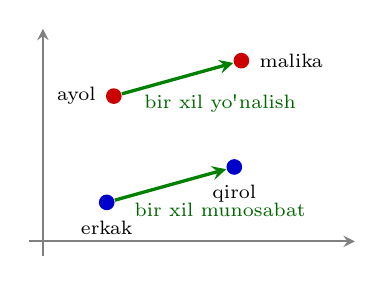
\begin{tikzpicture}[scale=0.9,>=stealth]
  \draw[->,thick,gray] (-0.2,0) -- (4.4,0);
  \draw[->,thick,gray] (0,-0.2) -- (0,3.0);

  \node[circle,fill=blue!80!black,inner sep=2pt,label=below:{\scriptsize erkak}] (m) at (0.9,0.55) {};
  \node[circle,fill=blue!80!black,inner sep=2pt,label=below:{\scriptsize qirol}] (k) at (2.7,1.05) {};

  \node[circle,fill=red!80!black,inner sep=2pt,label=left:{\scriptsize ayol}] (w) at (1.0,2.05) {};
  \node[circle,fill=red!80!black,inner sep=2pt,label=right:{\scriptsize malika}] (q) at (2.8,2.55) {};

  \draw[->,very thick,green!50!black] (m) -- (k);
  \draw[->,very thick,green!50!black] (w) -- (q);

  \node[green!40!black,font=\scriptsize] at (2.5,0.45)
       {bir xil munosabat};
  \node[green!40!black,font=\scriptsize] at (2.5,1.95)
       {bir xil yo\textquotesingle{}nalish};
\end{tikzpicture}
\end{column}

%------------------------------------------------
\begin{column}{0.46\textwidth}
\textbf{Asosiy g\textquotesingle{}oya}

\vspace{4pt}
\begin{itemize}\setlength\itemsep{5pt}
  \item Embedding fazosida ayrim semantik munosabatlar
        vektorlar orasidagi yo\textquotesingle{}nalish orqali namoyon bo\textquotesingle{}ladi.
  \item Masalan:
  \[
    E(\textit{qirol})-E(\textit{erkak})
    \approx
    E(\textit{malika})-E(\textit{ayol})
  \]
  \item Shu sababli so\textquotesingle{}z analogiyalarini vektor arifmetikasi
        orqali izohlash mumkin:
  \[
    \textit{king}-\textit{man}+\textit{woman}\approx \textit{queen}.
  \]
\end{itemize}

\vspace{3pt}
\footnotesize
Bu natija faqat sifatli va yetarli korpusda o\textquotesingle{}qitilgan embeddinglarda
aniqroq ko\textquotesingle{}rinadi.
\end{column}
\end{columns}

\end{frame}

% ----------------------------------------------------------------
% [G3] RASMIY TA'RIF: ANALOGIYA + BUNDA
% ----------------------------------------------------------------
\begin{frame}{So\textquotesingle{}z analogiyasi: rasmiy ta\textquotesingle{}rif}
\small

\begin{columns}[T,totalwidth=\textwidth]
%------------------------------------------------
\begin{column}{0.52\textwidth}

\textbf{Analogiya savoli}

\vspace{3pt}
\[
a:b::c:?
\]

\footnotesize
Mazmuni: “$a$ ga $b$ qanday munosabatda bo\textquotesingle{}lsa,
$c$ ga qaysi so\textquotesingle{}z shunday munosabatda?”

\vspace{6pt}

\begin{tcolorbox}[defbox]
\[
\mathbf{t}
=
\mathbf{b}-\mathbf{a}+\mathbf{c}
\]
\footnotesize
$\mathbf{t}$ — javob so\textquotesingle{}z emas, balki qidiriladigan
so\textquotesingle{}zga mos \textbf{maqsad vektor}.
\end{tcolorbox}

\vspace{4pt}

\[
\hat{d}
=
\arg\max_{w\in V\setminus\{a,b,c\}}
\cos\bigl(E(w),\mathbf{t}\bigr)
\]

\end{column}

%------------------------------------------------
\begin{column}{0.44\textwidth}

\textbf{Formula qanday o\textquotesingle{}qiladi?}

\vspace{4pt}
\begin{itemize}\setlength\itemsep{5pt}
  \item $\mathbf{b}-\mathbf{a}$ — “$a$ dan $b$ ga” semantik siljish.
  \item Shu siljish $\mathbf{c}$ ga qo\textquotesingle{}shiladi.
  \item $\mathbf{t}$ ga eng yaqin so\textquotesingle{}z kosinus orqali topiladi.
\end{itemize}

\vspace{5pt}

\begin{tcolorbox}[defbox]
\footnotesize
Masalan:
\[
\textit{king}-\textit{man}+\textit{woman}
\approx
\textit{queen}.
\]
\end{tcolorbox}

\vspace{3pt}
\footnotesize
Amaliy kutubxonalarda bu g\textquotesingle{}oya ko\textquotesingle{}pincha
\texttt{most\_similar} funksiyasi orqali bajariladi.

\end{column}
\end{columns}

\end{frame}

\begin{frame}{Analogiyani 2D vektorlarda qo\textquotesingle{}lda yechish}
\scriptsize

\begin{columns}[T,totalwidth=\textwidth]
%------------------------------------------------
\begin{column}{0.52\textwidth}

\textbf{Analogiya savoli}
\[
\textit{O\textquotesingle{}zbekiston}:\textit{Toshkent}
\;::\;
\textit{Rossiya}:?
\]

{\scriptsize \textit{Izoh: sonlar haqiqiy embedding emas, mexanizmni
tushuntirish uchun berilgan 2D misoldir.}}

\vspace{2pt}

\begin{tcolorbox}[defbox,left=2mm,right=2mm,top=1mm,bottom=1mm]
\[
E(\textit{O\textquotesingle{}zbekiston})=(2,0),\quad
E(\textit{Toshkent})=(3,1)
\]
\[
E(\textit{Rossiya})=(6,0),\quad
E(\textit{Moskva})=(7,1),\quad
E(\textit{Parij})=(9,5)
\]
\end{tcolorbox}

\vspace{1pt}

\textbf{1-qadam. Semantik siljishni topamiz}
\[
\Delta
=
E(\textit{Toshkent})-E(\textit{O\textquotesingle{}zbekiston})
=
(3,1)-(2,0)
=
(1,1)
\]

\vspace{1pt}

\textbf{2-qadam. Siljishni Rossiyaga qo\textquotesingle{}llaymiz}
\[
\mathbf{t}
=
E(\textit{Rossiya})+\Delta
=
(6,0)+(1,1)
=
(7,1)
=
E(\textit{Moskva})
\]

\[
\Rightarrow\quad \textbf{javob: Moskva.}
\]

\end{column}

%------------------------------------------------
\begin{column}{0.44\textwidth}
\centering

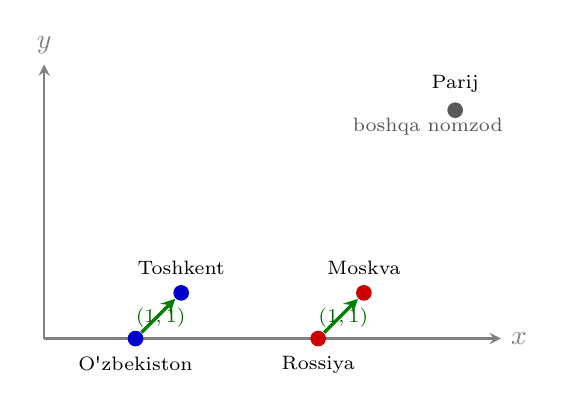
\begin{tikzpicture}[scale=0.58,>=stealth]
  \draw[->,thick,gray] (0,0) -- (10,0) node[right] {$x$};
  \draw[->,thick,gray] (0,0) -- (0,6) node[above] {$y$};

  \node[circle,fill=blue!80!black,inner sep=2pt,
        label=below:{\scriptsize O\textquotesingle{}zbekiston}] (uz) at (2,0) {};
  \node[circle,fill=blue!80!black,inner sep=2pt,
        label=above:{\scriptsize Toshkent}] (tosh) at (3,1) {};

  \node[circle,fill=red!80!black,inner sep=2pt,
        label=below:{\scriptsize Rossiya}] (ru) at (6,0) {};
  \node[circle,fill=red!80!black,inner sep=2pt,
        label=above:{\scriptsize Moskva}] (mos) at (7,1) {};

  \node[circle,fill=gray!70!black,inner sep=2pt,
        label=above:{\scriptsize Parij}] (par) at (9,5) {};

  \draw[->,very thick,green!50!black] (uz) -- (tosh);
  \draw[->,very thick,green!50!black] (ru) -- (mos);

  \node[green!40!black,font=\scriptsize] at (2.55,0.45) {$(1,1)$};
  \node[green!40!black,font=\scriptsize] at (6.55,0.45) {$(1,1)$};
  \node[gray!70!black,font=\scriptsize] at (8.4,4.65) {boshqa nomzod};
\end{tikzpicture}

\vspace{3pt}

\begin{tcolorbox}[defbox,left=2mm,right=2mm,top=1mm,bottom=1mm]
\scriptsize
Bir xil semantik siljish qo\textquotesingle{}llanadi:
\[
\textit{O\textquotesingle{}zbekiston}\rightarrow\textit{Toshkent},
\qquad
\textit{Rossiya}\rightarrow\textit{Moskva}.
\]
\end{tcolorbox}

\end{column}
\end{columns}

\end{frame}
% ----------------------------------------------------------------


% ----------------------------------------------------------------
% [J3] SIZNING VAZIFANGIZ: ANALOGIYA
% ----------------------------------------------------------------
\begin{frame}{Sizning vazifangiz: analogiyani yeching}
\small

\begin{columns}[T,totalwidth=\textwidth]
%------------------------------------------------
\begin{column}{0.48\textwidth}

\begin{tcolorbox}[alertbox,title=Vazifa]
\[
\textit{erkak}:\textit{qirol}
\;::\;
\textit{ayol}:?
\]

\[
E(\textit{erkak})=(1,1),\quad
E(\textit{qirol})=(3,2)
\]
\[
E(\textit{ayol})=(1,3)
\]

\[
E(\textit{malika})=(3,4),\quad
E(\textit{dehqon})=(2,1)
\]
\end{tcolorbox}

\end{column}

%------------------------------------------------
\begin{column}{0.48\textwidth}

\textbf{Yechim}

\[
\mathbf{t}
=
\mathbf{b}-\mathbf{a}+\mathbf{c}
=
(3,2)-(1,1)+(1,3)
=
(3,4)
\]

\vspace{3pt}

\[
\mathbf{t}=(3,4)=E(\textit{malika})
\]

\vspace{3pt}

\begin{tcolorbox}[defbox]
\footnotesize
\textbf{Javob:} \textit{malika}.  
Chunki \(\mathbf{t}\) vektori \textit{malika} vektori bilan aynan mos keladi;
\textit{dehqon} esa uzoqroq nomzod.
\end{tcolorbox}

\end{column}
\end{columns}

\end{frame}

% ----------------------------------------------------------------
% [K3] KOD <-> FORMULA: gensim most_similar  [fragile]
% ----------------------------------------------------------------
\begin{frame}[fragile]{Kod va formula: \texttt{most\_similar} orqali analogiya}
\scriptsize

\begin{columns}[T,totalwidth=\textwidth]
%------------------------------------------------
\begin{column}{0.55\textwidth}
\textbf{Gensim kodi}

\vspace{2pt}
\begin{tcolorbox}[defbox,left=2mm,right=2mm,top=1mm,bottom=1mm]
\begin{verbatim}
from gensim.models import KeyedVectors

wv = KeyedVectors.load("cc_uz_100k.kv")

# Eng yaqin so'zlar
wv.most_similar("toshkent", topn=3)

# Analogiya:
# O'zbekiston : Toshkent :: Rossiya : ?
wv.most_similar(
    positive=["toshkent", "rossiya"],
    negative=["uzbekiston"],
    topn=1
)

# Natija: [("moskva", 0.78)]
\end{verbatim}
\end{tcolorbox}
\end{column}

%------------------------------------------------
\begin{column}{0.41\textwidth}
\textbf{Formula bilan bog\textquotesingle{}lanishi}

\vspace{4pt}

\[
\mathbf{t}
=
E(\textit{Toshkent})
-
E(\textit{O\textquotesingle{}zbekiston})
+
E(\textit{Rossiya})
\]

\vspace{3pt}

\begin{center}
\begin{tabular}{@{}l l@{}}
\toprule
\textbf{Kod} & \textbf{Formula} \\
\midrule
\texttt{positive=[b,c]} & $+\mathbf{b}+\mathbf{c}$ \\
\texttt{negative=[a]} & $-\mathbf{a}$ \\
\texttt{most\_similar} & $\arg\max \cos$ \\
\bottomrule
\end{tabular}
\end{center}

\vspace{5pt}

\begin{tcolorbox}[defbox,left=2mm,right=2mm,top=1mm,bottom=1mm]
\footnotesize
\textbf{Muhim:} \texttt{positive} ro\textquotesingle{}yxatidagi vektorlar
qo\textquotesingle{}shiladi, \texttt{negative} ro\textquotesingle{}yxatidagilar
ayriladi. Natija maqsad vektorga eng yaqin so\textquotesingle{}z sifatida topiladi.
\end{tcolorbox}

\vspace{2pt}
\footnotesize
3-amaliyotda aynan shu API ishlatiladi.
\end{column}
\end{columns}

\end{frame}

% ================================================================
\section[Vizualizatsiya]{PCA (Principal Component Analysis) bilan vizualizatsiya}
% ================================================================

% ----------------------------------------------------------------
% [F4] INTUITSIYA: 300D NI KO'RA OLMAYMIZ
% ----------------------------------------------------------------
\begin{frame}{300 o\textquotesingle{}lchamli embeddingni qanday ko\textquotesingle{}ramiz?}
\small

\begin{columns}[T,totalwidth=\textwidth]
%------------------------------------------------
\begin{column}{0.47\textwidth}

\textbf{Muammo}

\vspace{3pt}
\begin{itemize}\setlength\itemsep{5pt}
  \item Embeddinglar odatda 100--300 o\textquotesingle{}lchamli bo\textquotesingle{}ladi.
  \item Inson esa 2D yoki 3D fazoni qulay ko\textquotesingle{}ra oladi.
  \item Shuning uchun yuqori o\textquotesingle{}lchamli vektorlarni 2D ga tushirish kerak.
\end{itemize}

\vspace{5pt}

\begin{tcolorbox}[defbox]
\footnotesize
\textbf{PCA} (\textit{Principal Component Analysis}) yuqori
o\textquotesingle{}lchamli nuqtalarni eng ko\textquotesingle{}p dispersiya
saqlanadigan 2 ta yo\textquotesingle{}nalishga proyeksiya qiladi.
\end{tcolorbox}

\end{column}

%------------------------------------------------
\begin{column}{0.49\textwidth}
\centering

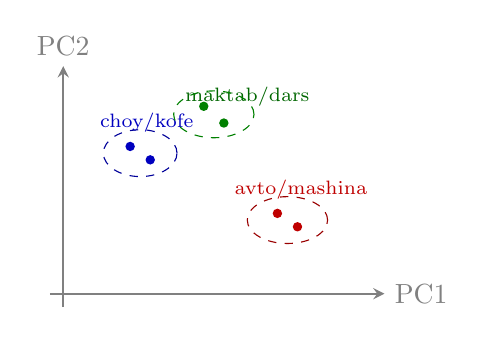
\begin{tikzpicture}[scale=0.85,>=stealth]
  \draw[->,thick,gray] (-0.2,0) -- (4.8,0) node[right] {PC1};
  \draw[->,thick,gray] (0,-0.2) -- (0,3.4) node[above] {PC2};

  \fill[blue!75!black] (1.0,2.2) circle (2pt);
  \fill[blue!75!black] (1.3,2.0) circle (2pt);
  \node[blue!75!black,font=\scriptsize] at (1.25,2.55) {choy/kofe};

  \fill[red!75!black] (3.2,1.2) circle (2pt);
  \fill[red!75!black] (3.5,1.0) circle (2pt);
  \node[red!75!black,font=\scriptsize] at (3.55,1.55) {avto/mashina};

  \fill[green!50!black] (2.1,2.8) circle (2pt);
  \fill[green!50!black] (2.4,2.55) circle (2pt);
  \node[green!40!black,font=\scriptsize] at (2.75,2.95) {maktab/dars};

  \draw[dashed,blue!60!black] (1.15,2.10) ellipse (0.55 and 0.35);
  \draw[dashed,red!60!black] (3.35,1.10) ellipse (0.60 and 0.35);
  \draw[dashed,green!50!black] (2.25,2.68) ellipse (0.60 and 0.35);
\end{tikzpicture}

\vspace{5pt}

\begin{tcolorbox}[alertbox]
\footnotesize
\textbf{Ehtiyot bo\textquotesingle{}ling:} PCA chizmasi taxminiy ko\textquotesingle{}rinish beradi.
Aniq yaqinlikni baholash uchun asl embedding fazosida kosinus hisoblanadi.
\end{tcolorbox}

\end{column}
\end{columns}

\end{frame}

% ----------------------------------------------------------------
% [G4] RASMIY TA'RIF: PCA (NAZARIY) + BUNDA
% ----------------------------------------------------------------
\begin{frame}{PCA: asosiy komponentlar tahlili}
\footnotesize

\begin{tcolorbox}[defbox,left=2mm,right=2mm,top=1mm,bottom=1mm]
\textbf{PCA} (\textit{Principal Component Analysis}) — yuqori o\textquotesingle{}lchamli
ma\textquotesingle{}lumotni dispersiya eng ko\textquotesingle{}p saqlanadigan yangi
o\textquotesingle{}qlarga proyeksiya qiluvchi o\textquotesingle{}lcham qisqartirish usuli.
\end{tcolorbox}

\vspace{3pt}

\begin{columns}[T,totalwidth=\textwidth]
\begin{column}{0.52\textwidth}

\textbf{Matematik g\textquotesingle{}oya}

\[
X_c = X-\bar{x}
\]

\[
C=\frac{1}{n-1}X_c^{\top}X_c
\]

\[
C\mathbf{v}_i=\lambda_i\mathbf{v}_i,
\qquad
\lambda_1\geq\lambda_2\geq\cdots
\]

\begin{itemize}\setlength\itemsep{3pt}
  \item $X_c$ — markazlashtirilgan ma\textquotesingle{}lumot;
  \item $C$ — kovariatsiya matritsasi;
  \item $\mathbf{v}_i$ — asosiy komponent yo\textquotesingle{}nalishi;
  \item $\lambda_i$ — shu yo\textquotesingle{}nalishdagi dispersiya.
\end{itemize}

\end{column}

\begin{column}{0.44\textwidth}
\centering

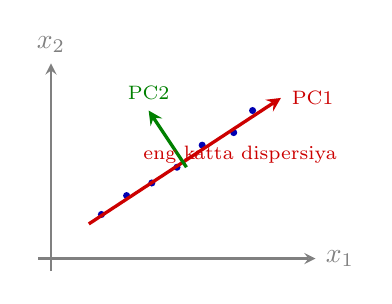
\begin{tikzpicture}[scale=0.80,>=stealth]
  \draw[->,thick,gray] (-0.2,0) -- (4.2,0) node[right] {$x_1$};
  \draw[->,thick,gray] (0,-0.2) -- (0,3.1) node[above] {$x_2$};

  \foreach \x/\y in {0.8/0.7,1.2/1.0,1.6/1.2,2.0/1.45,2.4/1.8,2.9/2.0,3.2/2.35}
    \fill[blue!70!black] (\x,\y) circle (1.6pt);

  \draw[->,very thick,red!80!black] (0.6,0.55) -- (3.65,2.55)
       node[right] {\scriptsize PC1};

  \draw[->,very thick,green!50!black] (2.15,1.45) -- (1.55,2.35)
       node[above] {\scriptsize PC2};

  \node[font=\scriptsize,red!80!black] at (3.0,1.65)
       {eng katta dispersiya};
\end{tikzpicture}

\vspace{4pt}

\begin{tcolorbox}[defbox,left=2mm,right=2mm,top=1mm,bottom=1mm]
\scriptsize
PC1 — dispersiya eng katta bo\textquotesingle{}lgan yo\textquotesingle{}nalish.  
PC2 — PC1 ga perpendikular keyingi asosiy yo\textquotesingle{}nalish.
\end{tcolorbox}

\end{column}
\end{columns}

\end{frame}

% ----------------------------------------------------------------
% [I4] QO'LDA MISOL: PCA INTUITSIYASI
% ----------------------------------------------------------------
\begin{frame}{Qo\textquotesingle{}lda misol: qaysi o\textquotesingle{}q ko\textquotesingle{}proq ma\textquotesingle{}lumot saqlaydi?}
\scriptsize

\begin{columns}[T,totalwidth=\textwidth]
%------------------------------------------------
\begin{column}{0.50\textwidth}

\textbf{Uchta markazlashtirilgan nuqta}

\[
\mathbf{w}_1=(2,0.1),\qquad
\mathbf{w}_2=(-2,-0.1),\qquad
\mathbf{w}_3=(0,0)
\]

\vspace{2pt}

\textbf{Har bir o\textquotesingle{}q bo\textquotesingle{}yicha tarqalish}

\[
\operatorname{Var}(x)\propto 2^2+(-2)^2+0^2=8
\]

\[
\operatorname{Var}(y)\propto 0.1^2+(-0.1)^2+0^2=0.02
\]

\[
\frac{\operatorname{Var}(x)}{\operatorname{Var}(y)}
=
\frac{8}{0.02}
=
400
\]

\vspace{2pt}

\begin{tcolorbox}[defbox,left=2mm,right=2mm,top=1mm,bottom=1mm]
\footnotesize
Demak, nuqtalar asosan $x$ o\textquotesingle{}qi bo\textquotesingle{}ylab
tarqalgan. PCA birinchi komponent sifatida shu yo\textquotesingle{}nalishni
saqlaydi.
\end{tcolorbox}

\end{column}

%------------------------------------------------
\begin{column}{0.46\textwidth}
\centering

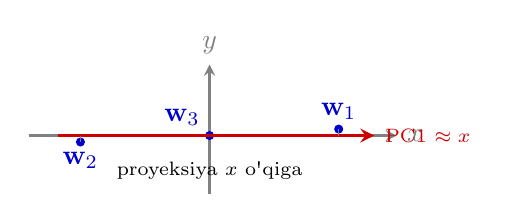
\begin{tikzpicture}[scale=0.82,>=stealth]
  \draw[->,thick,gray] (-2.8,0) -- (2.9,0) node[right] {$x$};
  \draw[->,thick,gray] (0,-0.9) -- (0,1.1) node[above] {$y$};

  \fill[blue!80!black] (2,0.1) circle (2pt);
  \node[blue!80!black,above] at (2,0.1) {$\mathbf{w}_1$};

  \fill[blue!80!black] (-2,-0.1) circle (2pt);
  \node[blue!80!black,below] at (-2,-0.1) {$\mathbf{w}_2$};

  \fill[blue!80!black] (0,0) circle (2pt);
  \node[blue!80!black,above left] at (0,0) {$\mathbf{w}_3$};

  \draw[->,very thick,red!80!black] (-2.35,0) -- (2.55,0)
       node[right] {\scriptsize PC1 $\approx x$};

  \draw[dashed,gray] (2,0.1) -- (2,0);
  \draw[dashed,gray] (-2,-0.1) -- (-2,0);

  \node[font=\scriptsize] at (0,-0.55) {proyeksiya $x$ o\textquotesingle{}qiga};
\end{tikzpicture}

\vspace{5pt}

\begin{tcolorbox}[alertbox,left=2mm,right=2mm,top=1mm,bottom=1mm]
\footnotesize
\[
\frac{8}{8+0.02}\approx 0.998
\]
Bitta komponent deyarli $99.8\%$ dispersiyani saqlaydi.
\end{tcolorbox}

\end{column}
\end{columns}

\end{frame}

% ----------------------------------------------------------------
% [J4] SIZNING VAZIFANGIZ: PCA NIMANI YO'QOTADI
% ----------------------------------------------------------------
\begin{frame}{PCA nimani saqlaydi, nimani yo\textquotesingle{}qotadi?}
\footnotesize

\begin{columns}[T,totalwidth=\textwidth]
%------------------------------------------------
\begin{column}{0.48\textwidth}

\begin{tcolorbox}[alertbox,title=Vazifa,left=2mm,right=2mm,top=1mm,bottom=1mm]
300 o\textquotesingle{}lchamli o\textquotesingle{}zbek embeddinglari PCA orqali
2D fazoga tushirildi:

\[
\texttt{explained\_variance\_ratio\_}=[0.31,\;0.18]
\]

\textbf{Savollar:}
\begin{enumerate}\setlength\itemsep{2pt}
  \item 2D tasvir ma\textquotesingle{}lumotning qancha qismini saqlaydi?
  \item 2D da yaqin ko\textquotesingle{}ringan so\textquotesingle{}zlar asl fazoda ham yaqin bo\textquotesingle{}lishi shartmi?
\end{enumerate}
\end{tcolorbox}

\end{column}

%------------------------------------------------
\begin{column}{0.48\textwidth}

\textbf{Yechim}

\[
0.31+0.18=0.49
\quad\Rightarrow\quad
49\%
\]

\[
1-0.49=0.51
\quad\Rightarrow\quad
51\%
\]

\begin{itemize}\setlength\itemsep{3pt}
  \item 2D proyeksiya dispersiyaning \textbf{49\%} qismini saqlaydi.
  \item Qolgan \textbf{51\%} dispersiya 2D tasvirda aks etmaydi.
  \item Shuning uchun 2D yaqinlik faqat taxminiy signal.
\end{itemize}

\vspace{2pt}

\begin{tcolorbox}[defbox,left=2mm,right=2mm,top=1mm,bottom=1mm]
\footnotesize
Aniq semantik yaqinlik asl embedding fazosida
kosinus o\textquotesingle{}xshashligi orqali baholanadi.
\end{tcolorbox}

\end{column}
\end{columns}

\end{frame}

% ----------------------------------------------------------------
% [K4] KOD <-> FORMULA: PCA + scatter  [fragile]
% ----------------------------------------------------------------
\begin{frame}[fragile]{Kod va formula: PCA bilan 2D vizualizatsiya}
\scriptsize

\begin{columns}[T,totalwidth=\textwidth]
%------------------------------------------------
\begin{column}{0.55\textwidth}
\textbf{Python kodi}

\vspace{2pt}
\begin{tcolorbox}[defbox,left=2mm,right=2mm,top=1mm,bottom=1mm]
\begin{verbatim}
from sklearn.decomposition import PCA
import matplotlib.pyplot as plt

# X: (N, d)  N ta so'z, d o'lchamli embedding
pca = PCA(n_components=2)

Z = pca.fit_transform(X)   # Z: (N, 2)

plt.scatter(Z[:, 0], Z[:, 1])

for i, word in enumerate(words):
    plt.annotate(word, Z[i])

print(pca.explained_variance_ratio_)
\end{verbatim}
\end{tcolorbox}
\end{column}

%------------------------------------------------
\begin{column}{0.41\textwidth}
\textbf{Formula bilan bog\textquotesingle{}lanishi}

\vspace{2pt}
\[
X_c = X-\bar{x}
\]

\[
Z = X_c
\begin{bmatrix}
\mathbf{v}_1 & \mathbf{v}_2
\end{bmatrix}
\]

\vspace{1pt}

\begin{tabular}{@{}l l@{}}
\toprule
\textbf{Kod} & \textbf{Ma\textquotesingle{}nosi} \\
\midrule
\texttt{n\_components=2} & PC1, PC2 \\
\texttt{fit\_transform(X)} & 2D proyeksiya \\
\texttt{Z[:,0]} & PC1 koordinata \\
\texttt{Z[:,1]} & PC2 koordinata \\
\texttt{annotate} & so\textquotesingle{}z yorlig\textquotesingle{}i \\
\bottomrule
\end{tabular}

\vspace{4pt}

\begin{tcolorbox}[defbox,left=2mm,right=2mm,top=1mm,bottom=1mm]
\scriptsize
\texttt{explained\_variance\_ratio\_} PC1 va PC2 qancha dispersiya
saqlaganini ko\textquotesingle{}rsatadi.
\end{tcolorbox}

\vspace{3pt}
\scriptsize
\textbf{Eslatma:} PCA chizmasi taxminiy talqin beradi; aniq yaqinlik
asl embedding fazosida kosinus orqali baholanadi.

\end{column}
\end{columns}

\end{frame}

% ================================================================
\section[Xulosa]{Xulosa va amaliyotga ko'prik}
% ================================================================

% ----------------------------------------------------------------
% [M] O'ZBEK TILIGA XOSLIK (majburiy arxetip)
% ----------------------------------------------------------------
\begin{frame}{O\textquotesingle{}zbek tili uchun embedding: qamrov, agglutinatsiya va subword}
\footnotesize

\begin{columns}[T,totalwidth=\textwidth]
%------------------------------------------------
\begin{column}{0.48\textwidth}

\textbf{Asosiy muammolar}

\begin{itemize}\setlength\itemsep{5pt}
  \item \textbf{Qamrov:} model lug\textquotesingle{}atida bo\textquotesingle{}lmagan
        so\textquotesingle{}zlar OOV muammosini keltirib chiqaradi.
  \item \textbf{Agglutinatsiya:} bitta ildizdan ko\textquotesingle{}plab shakllar hosil bo\textquotesingle{}ladi:
        \[
        \textit{kitob},\ \textit{kitoblar},\ \textit{kitoblarimizdan}.
        \]
  \item \textbf{Kam resurslilik:} katta, toza va balanslangan o\textquotesingle{}zbek korpuslari
        yetarli bo\textquotesingle{}lmasa, embedding sifati pasayadi.
\end{itemize}

\vspace{3pt}

\begin{tcolorbox}[alertbox,left=2mm,right=2mm,top=1mm,bottom=1mm]
\scriptsize
Bir xil ma\textquotesingle{}noga yaqin shakllar alohida token sifatida ko\textquotesingle{}rilsa,
ular orasidagi semantik bog\textquotesingle{}liqlik zaiflashadi.
\end{tcolorbox}

\end{column}

%------------------------------------------------
\begin{column}{0.48\textwidth}

\textbf{Amaliy yechimlar}

\begin{itemize}\setlength\itemsep{5pt}
  \item \textbf{Normalizatsiya:} imlo, apostrof, lotin-kiril yozuvi va tokenizatsiyani
        bir xil standartga keltirish.
  \item \textbf{Lemmatizatsiya/stemming:} so\textquotesingle{}z shakllarini umumiy ildiz yoki
        lemma atrofida birlashtirish.
  \item \textbf{Subword yondashuv:} FastText yoki BPE/WordPiece orqali so\textquotesingle{}zni
        kichik birliklarga ajratish.
\end{itemize}

\vspace{3pt}

\begin{tcolorbox}[defbox,left=2mm,right=2mm,top=1mm,bottom=1mm]
\scriptsize
Subword yondashuv OOV muammosini kamaytiradi: model butun so\textquotesingle{}zni
bilmasa ham, uning qismlaridan vektor hosil qilishi mumkin.
\end{tcolorbox}

\vspace{2pt}

\[
\textit{kitoblarimizdan}
\approx
\textit{kitob}+\textit{lar}+\textit{imiz}+\textit{dan}
\]

\end{column}
\end{columns}

\end{frame}

% ----------------------------------------------------------------
% [N] SINTEZ: SIYRAK vs ZICH TAQQOSLOV
% ----------------------------------------------------------------
\begin{frame}{Qachon nima ishlatamiz? Siyrak va zich vektorlar taqqoslovi}
\footnotesize

\begin{center}
\begin{tabular}{p{0.22\textwidth} p{0.34\textwidth} p{0.34\textwidth}}
\toprule
\textbf{Mezon} & \textbf{Siyrak vektorlar: BoW / TF-IDF} & \textbf{Zich vektorlar: embedding} \\
\midrule
Ifoda &
Juda katta o\textquotesingle{}lchamli, ko\textquotesingle{}p komponentalari nol. &
Kichik o\textquotesingle{}lchamli, komponentalari zich. \\[3pt]

Ma\textquotesingle{}no &
So\textquotesingle{}z chastotasi va hujjatdagi ahamiyatini aks ettiradi. &
Kontekst va semantik yaqinlikni ifodalashga harakat qiladi. \\[3pt]

Afzallik &
Sodda, tez, talqin qilish oson. Kichik datasetlarda yaxshi ishlaydi. &
Sinonimlik, yaqin ma\textquotesingle{}no va analogiyalarni yaxshiroq ushlaydi. \\[3pt]

Kamchilik &
Sinonimlarni va yashirin semantik bog\textquotesingle{}liqlikni ko\textquotesingle{}rmaydi. &
Ko\textquotesingle{}proq korpus, sifatli model va ehtiyotkor talqin talab qiladi. \\[3pt]

Qachon? &
Klassik tasniflash, qidiruv, baseline model. &
Semantik qidiruv, klasterlash, analogiya, transformer modellar.
\\
\bottomrule
\end{tabular}
\end{center}

\vspace{4pt}

\begin{tcolorbox}[defbox,left=2mm,right=2mm,top=1mm,bottom=1mm]
\scriptsize
Amaliy tavsiya: avval TF-IDF bilan kuchli baseline quriladi; semantik yaqinlik muhim bo\textquotesingle{}lsa,
embedding yoki transformer embeddinglariga o\textquotesingle{}tiladi.
\end{tcolorbox}

\end{frame}

% ----------------------------------------------------------------
% [O] SEMINAL MAQOLA + MUHOKAMA SAVOLI
% ----------------------------------------------------------------
\begin{frame}{Seminal maqola: GloVe (Pennington va b., 2014)}
\footnotesize

\begin{columns}[T,totalwidth=\textwidth]
%------------------------------------------------
\begin{column}{0.50\textwidth}

\textbf{Asosiy g\textquotesingle{}oya}

\begin{itemize}\setlength\itemsep{4pt}
  \item GloVe — \textit{Global Vectors for Word Representation}.
  \item Model butun korpus bo\textquotesingle{}yicha so\textquotesingle{}zlarning
        birga uchrashish statistikasi asosida o\textquotesingle{}rganadi.
  \item Faqat lokal kontekst emas, global \textit{co-occurrence} matritsasi ham hisobga olinadi.
\end{itemize}

\vspace{4pt}

\begin{tcolorbox}[defbox,left=2mm,right=2mm,top=1mm,bottom=1mm]
\scriptsize
GloVe g\textquotesingle{}oyasi: so\textquotesingle{}zlar orasidagi ma\textquotesingle{}no
farqi ularning turli kontekst so\textquotesingle{}zlari bilan uchrashish
nisbatlarida ko\textquotesingle{}rinadi.
\end{tcolorbox}

\end{column}

%------------------------------------------------
\begin{column}{0.46\textwidth}

\textbf{Model formulasi}

\[
J=
\sum_{i,j=1}^{|V|}
f(X_{ij})
\bigl(
\mathbf{w}_i^{\top}\tilde{\mathbf{w}}_j
+
b_i+\tilde{b}_j
-
\log X_{ij}
\bigr)^2
\]

\vspace{2pt}

\begin{itemize}\setlength\itemsep{3pt}
  \item $X_{ij}$ — $i$ va $j$ so\textquotesingle{}zlarining birga uchrashish soni;
  \item $\mathbf{w}_i$, $\tilde{\mathbf{w}}_j$ — o\textquotesingle{}rganiladigan vektorlar;
  \item $f(X_{ij})$ — juda kam yoki juda ko\textquotesingle{}p uchrashlarni muvozanatlaydi.
\end{itemize}

\vspace{2pt}

\begin{tcolorbox}[alertbox,left=2mm,right=2mm,top=1mm,bottom=1mm]
\scriptsize
Amaliy talqin: GloVe katta va toza korpusda yaxshi ishlaydi;
kichik yoki shovqinli korpusda natija barqaror bo\textquotesingle{}lmasligi mumkin.
\end{tcolorbox}

\end{column}
\end{columns}

\end{frame}

% ----------------------------------------------------------------
% [P] MAQSADLAR BAJARILDI
% ----------------------------------------------------------------
\begin{frame}{Bugungi maqsadlar bajarildi}
\footnotesize

\begin{columns}[T,totalwidth=\textwidth]
%------------------------------------------------
\begin{column}{0.50\textwidth}

\textbf{Bugun nimalarni tushundik?}

\begin{itemize}\setlength\itemsep{5pt}
  \item TF-IDF semantik yaqinlikni har doim ham ifodalay olmasligini ko\textquotesingle{}rdik.
  \item So\textquotesingle{}z embeddingi $E:V\rightarrow \mathbb{R}^{d}$ sifatida ta\textquotesingle{}riflandi.
  \item Kosinus o\textquotesingle{}xshashligi orqali vektorlar yo\textquotesingle{}nalishi taqqoslandi.
  \item So\textquotesingle{}z analogiyasi $t=b-a+c$ orqali tushuntirildi.
\end{itemize}

\end{column}

%------------------------------------------------
\begin{column}{0.46\textwidth}

\textbf{Amaliy bog\textquotesingle{}lanish}

\begin{itemize}\setlength\itemsep{5pt}
  \item \texttt{cosine\_similarity} — vektorlar o\textquotesingle{}xshashligini hisoblaydi.
  \item \texttt{most\_similar} — maqsad vektorga eng yaqin so\textquotesingle{}zni topadi.
  \item PCA embeddinglarni 2D fazoda ko\textquotesingle{}rishga yordam beradi.
\end{itemize}

\vspace{4pt}

\begin{tcolorbox}[defbox,left=2mm,right=2mm,top=1mm,bottom=1mm]
\scriptsize
\textbf{Muhim xulosa:} PCA faqat vizual talqin beradi;
aniq semantik yaqinlik asl embedding fazosida kosinus orqali baholanadi.
\end{tcolorbox}

\end{column}
\end{columns}

\end{frame}

% ----------------------------------------------------------------
% [Q] KO'PRIK: ERTAGA P3
% ----------------------------------------------------------------
\begin{frame}{3-amaliyot: tayyor embeddinglar bilan ishlash}
\footnotesize

\begin{columns}[T,totalwidth=\textwidth]
%------------------------------------------------
\begin{column}{0.48\textwidth}

\textbf{Amaliyotda bajariladigan ishlar}

\begin{enumerate}\setlength\itemsep{5pt}
  \item Tayyor embedding modelini yuklash.
  \item So\textquotesingle{}z vektorini olish va uning o\textquotesingle{}lchamini tekshirish.
  \item Ikki so\textquotesingle{}z orasidagi kosinus o\textquotesingle{}xshashligini hisoblash.
  \item \texttt{most\_similar} orqali eng yaqin so\textquotesingle{}zlarni topish.
  \item PCA yordamida tanlangan so\textquotesingle{}zlarni 2D fazoda ko\textquotesingle{}rsatish.
\end{enumerate}

\vspace{3pt}

\begin{tcolorbox}[defbox,left=2mm,right=2mm,top=1mm,bottom=1mm]
\scriptsize
Asosiy e\textquotesingle{}tibor modelni qayta o\textquotesingle{}qitishga emas,
tayyor embedding vektorlari bilan to\textquotesingle{}g\textquotesingle{}ri ishlashga qaratiladi.
\end{tcolorbox}

\end{column}

%------------------------------------------------
\begin{column}{0.48\textwidth}

\textbf{Kutiladigan natijalar}

\begin{itemize}\setlength\itemsep{5pt}
  \item \textit{choy}--\textit{kofe}, \textit{avtomobil}--\textit{mashina}
        kabi juftliklarda yaqinlikni tekshirasiz.
  \item OOV so\textquotesingle{}zlar va apostrof/imlo farqlari model natijasiga
        qanday ta\textquotesingle{}sir qilishini ko\textquotesingle{}rasiz.
  \item PCA chizmasida semantik guruhlar qanday ko\textquotesingle{}rinishini
        tahlil qilasiz.
\end{itemize}

\vspace{4pt}

\begin{tcolorbox}[alertbox,left=2mm,right=2mm,top=1mm,bottom=1mm]
\scriptsize
\textbf{Ehtiyot bo\textquotesingle{}ling:} 2D PCA chizmasi faqat vizual yordam.
Yakuniy xulosa asl embedding fazosidagi kosinus o\textquotesingle{}xshashligi
asosida beriladi.
\end{tcolorbox}

\end{column}
\end{columns}

\end{frame}

% ----------------------------------------------------------------
% [R] ADABIYOTLAR
% ----------------------------------------------------------------
\begin{frame}{Adabiyotlar}
  \begin{enumerate}\small\setlength\itemsep{6pt}
    \item Pennington, J., Socher, R., Manning, C.D.\ (2014).
          \textit{GloVe: Global Vectors for Word Representation.}
          EMNLP 2014.
    \item Mikolov, T. va b.\ (2013).
          \textit{Efficient Estimation of Word Representations in
          Vector Space.} ICLR 2013. (Word2Vec --- L6 da batafsil.)
    \item Jurafsky, D., Martin, J.H.\ (2023).
          \textit{Speech and Language Processing}, 3-nashr (online).
          6-bob: Vector Semantics and Embeddings.
    \item Firth, J.R.\ (1957). \textit{A Synopsis of Linguistic Theory.}
          (Distributiv gipoteza manbasi.)
    \item Scikit-learn hujjatlari: \texttt{cosine\_similarity},
          \texttt{PCA} --- scikit-learn.org.
  \end{enumerate}
\end{frame}

% ================================================================
% [S] ILOVALAR (appendix --- slayd soniga kirmaydi)
% ================================================================
\appendix

\begin{frame}{Ilova S1: kosinus va Evklid masofa bog'liqligi}
  \small
  $L_2$-normallashtirilgan vektorlar uchun
  ($\lVert\mathbf{a}\rVert=\lVert\mathbf{b}\rVert=1$):
  $$\lVert\mathbf{a}-\mathbf{b}\rVert^2
    = \lVert\mathbf{a}\rVert^2 + \lVert\mathbf{b}\rVert^2
      - 2\,\mathbf{a}\cdot\mathbf{b}
    = 2 - 2\cos(\mathbf{a},\mathbf{b})$$
  \vspace{-2pt}
  \begin{columns}[T]
    \begin{column}{0.54\textwidth}
      \bunda{$\lVert\mathbf{a}\rVert=\lVert\mathbf{b}\rVert=1$ deb olindi.}
      \vspace{5pt}

      Demak normallashtirilgan fazoda Evklid masofasi va kosinus
      \textbf{ekvivalent tartib} beradi --- shuning uchun ko'p kutubxonalar
      ikkalasini almashtirib ishlatadi. Bu LSH va qidiruvda muhim (L4, P4).
    \end{column}
    \begin{column}{0.44\textwidth}
      \centering
      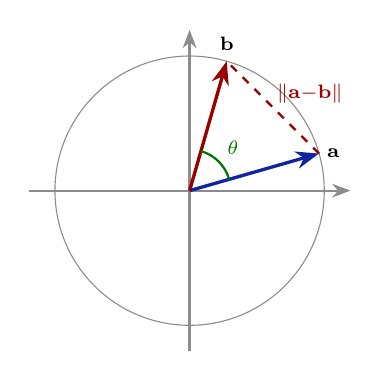
\begin{tikzpicture}[scale=0.95,>=Stealth,font=\scriptsize]
        \draw[halfgray,thin] (0,0) circle (1.8);
        \draw[axisline] (-2.15,0) -- (2.15,0);
        \draw[axisline] (0,-2.15) -- (0,2.15);
        \draw[vecA] (0,0) -- (16:1.8) node[right=-1pt]{$\mathbf{a}$};
        \draw[vecB] (0,0) -- (74:1.8) node[above]{$\mathbf{b}$};
        \draw[deepred,thick,dashed] (16:1.8) -- (74:1.8)
          node[midway,above right,inner sep=1pt]{$\lVert\mathbf{a}{-}\mathbf{b}\rVert$};
        \draw[deepgreen,thick] (16:0.55) arc (16:74:0.55);
        \node[deepgreen] at (45:0.82) {$\theta$};
      \end{tikzpicture}\\[2pt]
      \gcap{Birlik aylanada: vatar $=\lVert\mathbf{a}{-}\mathbf{b}\rVert$, burchak $\theta$}
    \end{column}
  \end{columns}
\end{frame}

\begin{frame}{Ilova S2: vektor, norma va skalyar ko'paytma eslatmasi}
  \begin{columns}[T]
    \begin{column}{0.55\textwidth}
      \begin{tcolorbox}[defbox,title=Kerakli tushunchalar,top=2pt,bottom=2pt]
        \small
        Skalyar ko'paytma: $\mathbf{a}\cdot\mathbf{b}=\sum_i a_i b_i$\\[3pt]
        Evklid normasi (uzunlik): $\lVert\mathbf{a}\rVert=\sqrt{\sum_i a_i^2}$\\[3pt]
        Perpendikular vektorlar: $\mathbf{a}\cdot\mathbf{b}=0$
      \end{tcolorbox}
      \vspace{4pt}
      \small\textbf{Misol:} $\mathbf{a}=(3,4)$ uchun
      $\lVert\mathbf{a}\rVert=\sqrt{9+16}=\sqrt{25}=5$.\\[5pt]
      Python da: \texttt{np.linalg.norm([3,4])} $\to 5.0$;\\[2pt]
      \texttt{np.dot(a, b)} --- skalyar ko'paytma.
    \end{column}
    \begin{column}{0.43\textwidth}
      \centering
      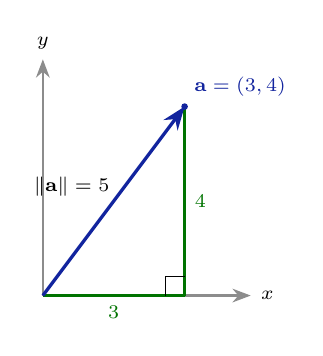
\begin{tikzpicture}[scale=0.6,>=Stealth,font=\scriptsize]
        \draw[axisline] (0,0) -- (4.4,0) node[right]{$x$};
        \draw[axisline] (0,0) -- (0,5.0) node[above]{$y$};
        \draw[deepgreen,thick] (0,0) -- (3,0) node[midway,below]{$3$};
        \draw[deepgreen,thick] (3,0) -- (3,4) node[midway,right]{$4$};
        \draw[vecA] (0,0) -- (3,4)
          node[midway,above left,inner sep=1pt]{$\lVert\mathbf{a}\rVert=5$};
        \draw (2.6,0) -- (2.6,0.4) -- (3,0.4);
        \fill[cnublue] (3,4) circle (2pt) node[above right]{$\mathbf{a}=(3,4)$};
      \end{tikzpicture}\\[2pt]
      \gcap{Norma $=$ gipotenuza $=\sqrt{3^2+4^2}=5$}
    \end{column}
  \end{columns}
\end{frame}

\begin{frame}{Ilova S3: PCA matematik asoslari}
  \begin{enumerate}\small\setlength\itemsep{5pt}
    \item Ma'lumotni markazlashtiring: har ustundan o'rtachani ayiring.
    \item Kovariatsiya matritsasi: $C=\frac{1}{n}X^\top X$.
    \item $C$ ning xos qiymat va xos vektorlarini toping.
    \item Eng katta $k$ xos qiymatga mos xos vektorlarni tanlang ---
          bular asosiy komponentlar.
    \item Ma'lumotni shu $k$ vektorga proyeksiya qiling.
  \end{enumerate}
  \vspace{4pt}
  \footnotesize\color{halfgray}
  \texttt{explained\_variance\_ratio\_[i]} $=\lambda_i / \sum_j \lambda_j$,
  bunda $\lambda_i$ --- $i$-xos qiymat. Bu kursda PCA ni \texttt{sklearn}
  amalga oshiradi --- qo'lda xos qiymat hisoblanmaydi.
\end{frame}

\end{document}
